\subsection{Software}
\subsubsection{Determining a 3D Model of an Object From a Video}
\subsubsection{Object Oriented vs. Procedural Neural Network Design}
\subsubsection{Feature Extraction}
In constellation's implementation, there are three main parts of extracting features from a two dimensional image; the first is training our system to recognize the object
\begin{figure}[h]
\centering
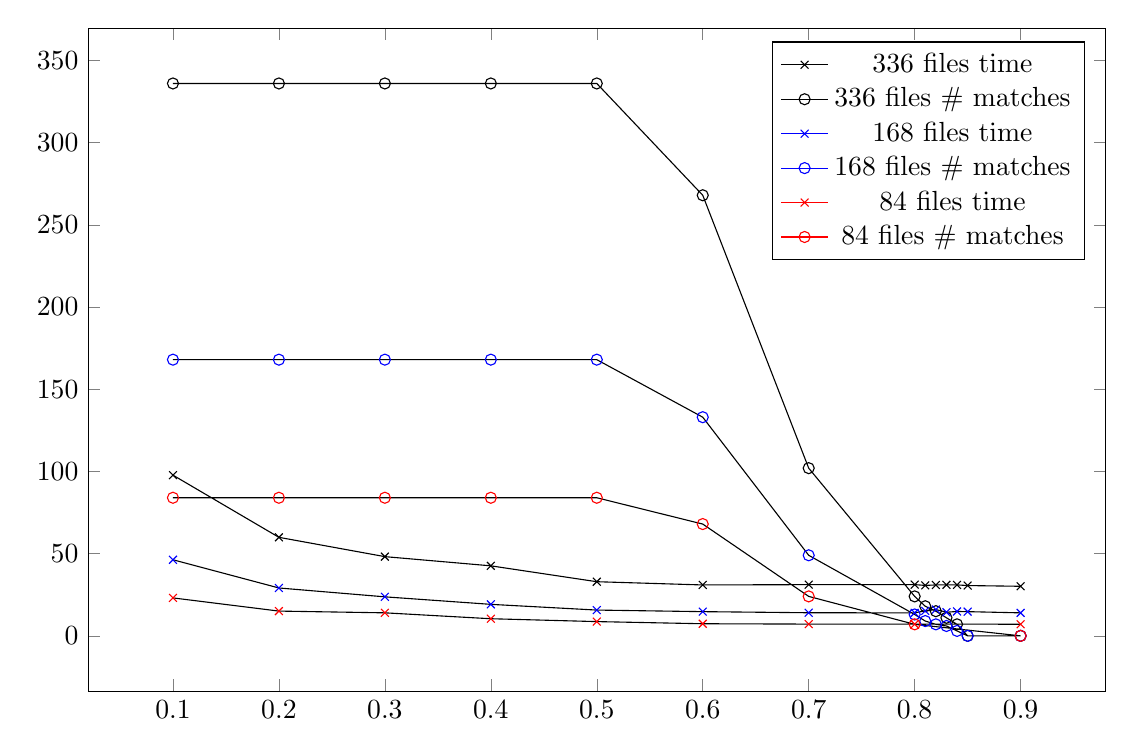
\begin{tikzpicture}
\begin{axis}[%
scatter/classes={%
    a={mark=x,draw=black},
    c={mark=o,draw=black},
    b={mark=x,draw=blue},
    d={mark=o,draw=blue},
    e={mark=x,draw=red},
    f={mark=o,draw=red}},width=14.5cm,height=10cm]
\addplot[scatter,%
    scatter src=explicit symbolic]%
table[meta=label] {
x y label
0.1 97.75 a
0.2 59.93 a
0.3 48.18 a
0.4 42.59 a
0.5 32.93 a
0.6 30.96 a
0.7 31.15 a
0.8 31.16 a
0.81 30.68 a
0.82 30.96 a
0.83 31.06 a
0.84 30.99 a
0.85 30.59 a
0.9 30.15 a

0.1 336 c
0.2 336 c
0.3 336 c
0.4 336 c
0.5 336 c
0.6 268 c
0.7 102 c
0.8 24 c
0.81 18 c
0.82 15 c
0.83 11 c
0.84 7 c
0.85 0 c
0.9 0 c

0.1 46.28 b
0.2 29.12 b
0.3 23.73 b
0.4 19.16 b
0.5 15.68 b
0.6 14.72 b
0.7 14.05 b
0.8 13.98 b
0.81 15.22 b
0.82 16 b
0.83 14.37 b
0.84 14.82 b
0.85 14.72 b
0.9 13.99 b

0.1 168 d
0.2 168 d
0.3 168 d
0.4 168 d
0.5 168 d
0.6 133 d
0.7 49 d
0.8 13 d
0.81 9 d
0.82 7 d
0.83 6 d
0.84 3 d
0.85 0 d
0.9 0 d

0.1 23.08 e
0.2 15.06 e
0.3 14.00 e
0.4 10.41 e
0.5 8.67 e
0.6 7.36 e
0.7 7.15 e
0.8 7.12 e
0.9 7.08 e

0.1 84 f
0.2 84 f
0.3 84 f
0.4 84 f
0.5 84 f
0.6 68 f
0.7 24 f
0.8 7 f
0.9 0 f
    };
\addlegendentry{336 files time}
\addlegendentry{336 files \# matches}
\addlegendentry{168 files time}
\addlegendentry{168 files \# matches}
\addlegendentry{84 files time}
\addlegendentry{84 files \# matches}
\end{axis}
\end{tikzpicture}
\caption{Number of Matches Found (number) and Speed of Matching (seconds) vs. Confidence Level For Varying Amounts of Training Images}
\end{figure}
\subsubsection{Distance Estimation}
\subsubsection{Environment Model Generation}
\subsubsection{User-Facing Application}